\documentclass{astroedu-lab}

\begin{document}

\pagestyle{plain}

\begin{problem}{\huge Лабораторная работа 4.2.4\\\\Интерферометр Майкельсона\\\\Выполнил Жданов Елисей Б01-205}

\section{Цель работы:}

1) Изучение двухлучевой интерференции

2) Определение длины волны

3) Проверка эффекта Доплера

\section{Оборудование:}

1) интерферометр Майкельсона с подвижным зеркалом

2) лазер

3) фотоумножитель

4) частотомер

5) линзы

\section{Теоретическая справка}

Схема интерферометра приведена на рис. 1. В этом интерферометре когерентные волны получаются методом деления амплитуды при использовании полупрозрачного зеркала ПП. Интерференционная картина наблюдается в плоскости экрана Э. Источником света является точка, получающаяся за счёт фокусировки лазерного излучения с помощью дополнительной линзы. В данной схеме интерференции требуется большая временная когерентность, поэтому используется лазерный источник излучения.

Картина интерференции на экране Э может быть построена следующим образом. Отражаясь в зеркалах ПП, $3_1$ и $3_2$, источник $S$ даёт два изображения $S_1$ и $S_2$ (рис. 2.22). Если зеркало $3_2$ не перпендикулярно падающему лучу $2, S_2$ переходит в $S_2^{\prime}$. То есть интерференцию на экране можно рассматривать как интерференцию от двух точечных источников.

Если экран расположен перпендикулярно линии, соединяющей два источника, линиями равной разности фаз будут окружности
$$
\sqrt{L^2+r_n^2}-\sqrt{(L-a)^2+r_n^2} \approx a+\frac{r^2 a}{2 L(L-a)}=\text { const },
$$

\begin{figure}[!h]
	\centering
	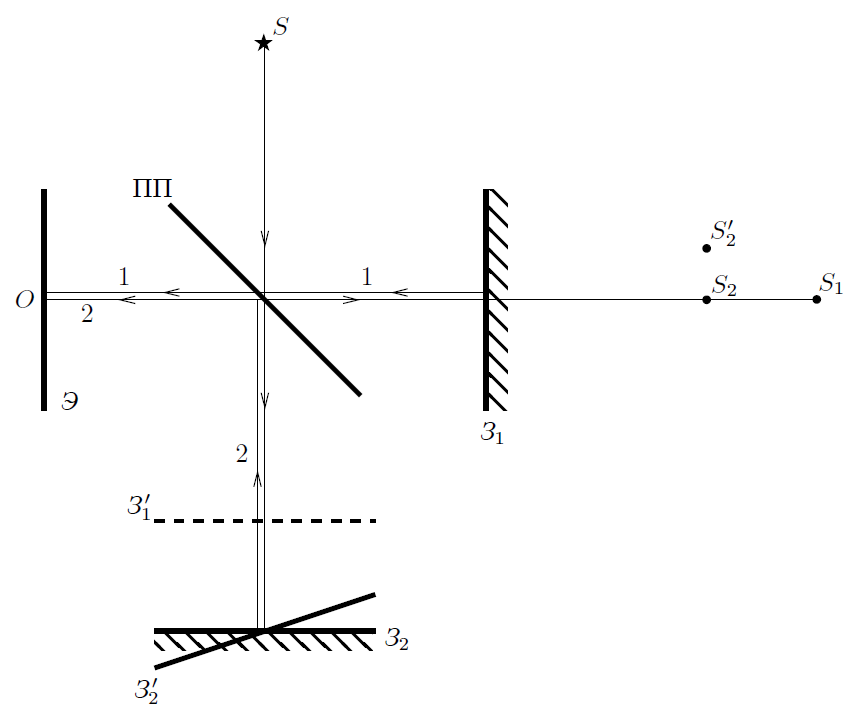
\includegraphics[width=0.7\textwidth]{теоруст.png}
	\caption{Схема интерферометра}
	\label{fig:boiler}
\end{figure}

где $r_n$ - радиус окружности, $a$ - расстояние между изображениями источника $S$, а $L$ - расстояние от $S_1$ до экрана.

Интенсивность в центре картины ( $r=0$ ) определяется величиной $a$, равной разности хода между лучами 1 и 2. Порядок интерференции в центре равен $m_0=\frac{a}{\lambda}$. Если в центре имеется максимум, тогда радиус $n$-го интерференционного кольца, отсчитанного от центра, будет определяться формулой
$$
r_n \approx \sqrt{\frac{2 n L(L-a)}{m_0}},
$$

где $n=0,1,2 \ldots$ При больших $n$ расстояние между полосами будет равно
$$
\Delta r \approx \sqrt{\frac{L(L-a)}{2 n m_0}} .
$$






При малом повороте зеркала $3_2$ изображение источника $S_2$ переходит в $S_2^{\prime}$. Если от центра экрана изображения источников будут видны под углом $\beta$, то в центре будут видны полосы, ширина которых согласно (2.25) приближенно равна $\lambda / \beta$.

По интерференционной картине можно определять длину волны источника света. При движении зеркала $3_1$ к экрану (зеркало $3_2$ установлено без наклона) разность хода со временем уменьшается, интерференционные кольца стягиваются к центру, как бы исчезая в нём. При смещении зеркала на расстояние $l$ в центре исчезнет $N=2 \frac{l}{\lambda}$ колец. При равномерном перемещении зеркала, если за время $T$ зарегистрировано исчезновение $N$ колец, скорость перемещения зеркала равна
$$
v=\frac{\lambda}{2} \frac{N}{T} .
$$

Для более точного рассмотрения необходимо воспользоваться релятивистскими формулами для эффекта Доплера. Учтём, что в системе координат, связанной с зеркалом $3_1$, движущимся со скоростью $v$, частота излучения источника $\omega_1$ отличается от исходной $\omega_0$, так что $\omega_1=\omega_0 \sqrt{\frac{c+v}{c-v}}$. Эта волна отражается от неподвижного зеркала и попадает на движущийся (в системе зеркала) приёмник. Частота приёма будет равна $\omega_2=\omega_1 \sqrt{\frac{c+v}{c-v}}=\omega_0 \frac{c+v}{c-v}$. В центре экрана колебания $\omega_0$ и $\omega_2$ складываются, и регистрируемая интенсивность меняется с частотой $\Delta \omega=\frac{2 v}{c-v} \omega_0$. Число периодов колебаний за время $t$ равно
$$
N=\frac{\Delta \omega t}{2 \pi}=2 \frac{v t}{\lambda} \frac{1}{1-\frac{v}{c}} .
$$

Для небольших скоростей эта формула совпадает с (2.70).


\section{Экспериментальная установка}


Схема устройства интерферометра приведена на рис. 1. Источником света служит лазер ЛГ. Лазер излучает узкий пучок света, который фокусируется линзой Л$_1$. В фокусе этой линзы возникает точечный источник света 5. Сферическая световая волна от источника 5 падает на делительную призму П и делится её диагональной гранью на две волны --- отражённую 1 и проходящую 2. Волна 1 отражается от зеркала З$_1$, возвращается к призме П, частично проходит сквозь неё и попадает на экран Э. Волна 2 отражается от зеркала 3$_2$, частично отражается от призмы П и также попадает на экран. Световые волны 1 и 2 испускаются одним источником 5, и они когерентны между собой. Эти волны создают на экране Э интерференционную картину. Для увеличения масштаба интерференционной картины может быть использована линза Л$_2$.
	
		\begin{figure}[h]
		\begin{center}
			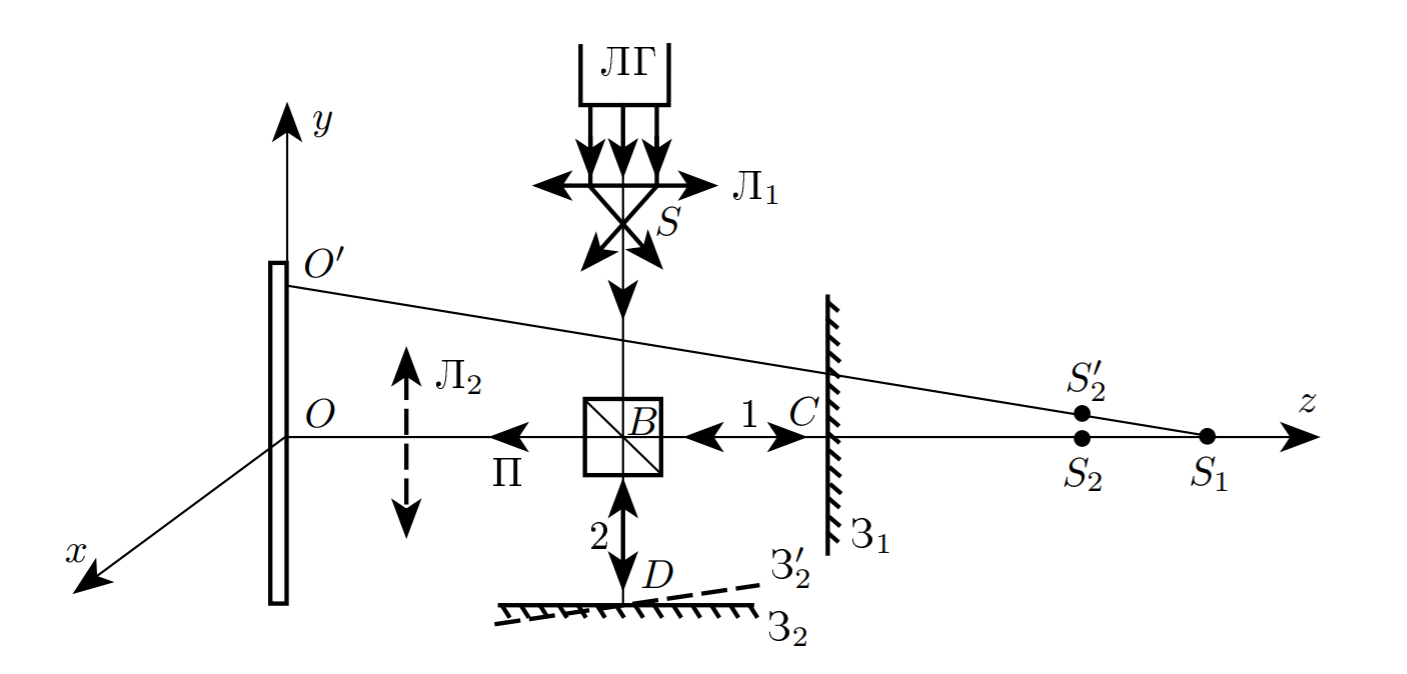
\includegraphics[width = 0.7\textwidth]{424-1.png}
			\caption{Схема интерферометра}
		\end{center}
	\end{figure}
	
	Зеркало З$_1$ установлено перпендикулярно падающему лучу. Оно может перемещаться вдоль луча. Это зеркало в дальнейшем будет называться подвижным. Зеркало 3$_2$ вдоль направления падающего луча не перемещается. Его, однако, можно наклонять по отношению к лучу.
	
	Схема экспериментальной установки приведена на рис. 2. Источником света служит гелий-неоновый лазер ЛГН-203. Его излучение обладает большой длиной когерентности, что позволяет получать хорошо различимую глазом интерференционную картину при разности хода в десятки сантиметров. Неподвижное зеркало 3$_2$, поворачивается микрометрическими винтами М, (относительно горизонтальной) и М, (относительно вертикальной оси). Зеркало З$_1$ установлено перпендикулярно падающему лучу.
	\begin{figure}[h]
		\begin{center}
			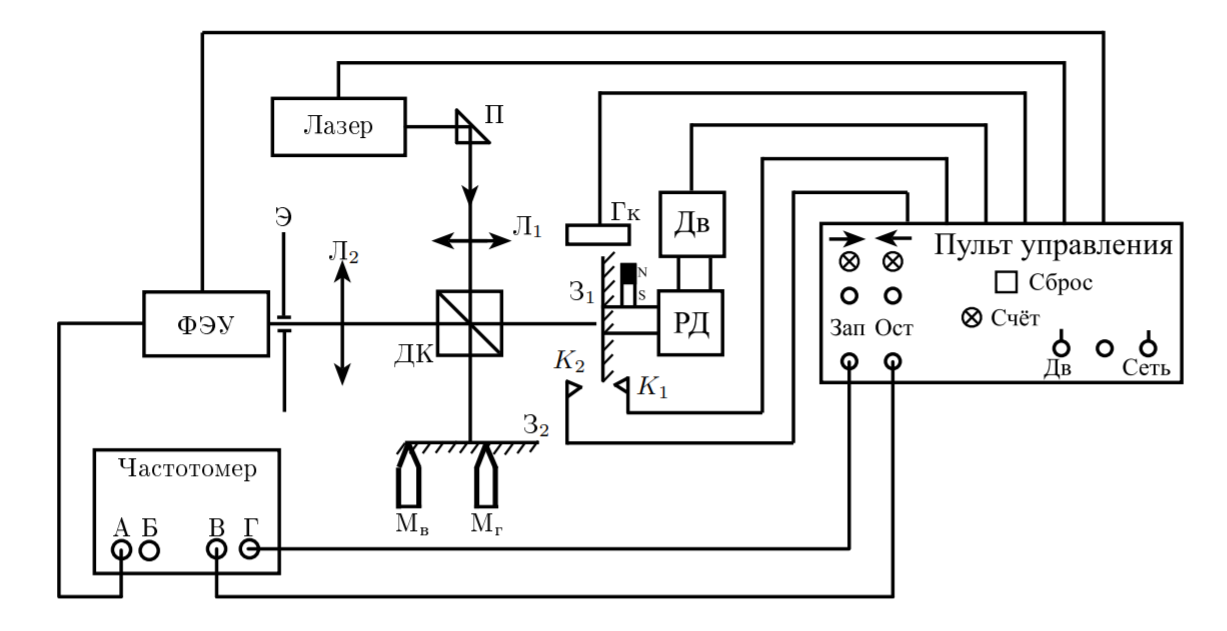
\includegraphics[width = 0.85\textwidth]{424-2.png}
			\caption{Схема установки}
		\end{center}
	\end{figure}
	 Оно может передвигаться вдоль луча с помощью микрометрического винта, соединённого с двигателем Дв через муфту и редуктор РД, позволяющий менять скорость движения зеркала. Двигатель питается от сети через блок питания пульта управления. Концевые контакты К$_1$ и К$_2$ меняют направление движения зеркала на обратное. Включение лазера и двигателя производится с пульта управления. Сигнальные лампочки указывают, в какую сторону движется зеркало.
	 
	 Интерференционная картина наблюдается на экране Э. Она может быть увеличена с помощью линзы Л$_2$. В этом случае на экране в увеличенном масштабе воспроизводится интерференционная картина, которая создаётся перед линзой в плоскости, сопряжённой экрану. Линза закреплена на съёмном столике, её фокусное расстояние 4,3 см.
	 
	 Для регистрации изменения интенсивности света используется фотоэлектронный умножитель ФЭУ-68, установленный непосредственно за экраном. Свет на окно ФЭУ попадает через небольшое отверстие в центре экрана. Для питания ФЭУ используется высоковольтный выпрямитель. Выпрямитель включается тумблером «Сеть» на пульте управления.
	 
	 Периодическое изменение интенсивности света, возникающее при движении зеркала З1, приводит к такому же изменению сигнала ФЭУ. Число периодов изменения интенсивности света пересчитывается частотомером Ч3-54. Частотомер может работать в одном из трёх режимов.
	 \begin{enumerate}
	 	\item Он может измерять число импульсов, поступающих на его входы (А или Б) за некоторый промежуток времени (его продолжительность определяется поступлением сигналов на управляющие входы В и Г).
	 	\item С помощью частотомера можно измерять промежутки времени. Для таких измерений в прибор встроен кварцевый генератор. Частотомер измеряет время, прошедшее между поступлением сигналов на его управляющие входы, подсчитывая соответствующее число импульсов кварцевого генератора.
	 	\item Наконец, частотомер может измерять частоту сигнала, поступающего на его вход, сравнивая число периодов исследуемого сигнала с числом импульсов кварцевого генератора. 
	 	
 	\end{enumerate}
	 	
	 	Для получения управляющих сигналов используется геркон Гк (герметичный магнитоуправляемый контакт). Схема работает следующим образом. На отсчётной головке микрометрического винта зеркала З$_1$ закреплён небольшой магнит. Головка вращается вместе с винтом. После срабатывания концевого контакта. К$_2$ зеркало начинает двигаться от экрана. При приближении магнита к геркону вырабатывается управляющий сигнал, который подаётся через схему пульта управления на вход В частотомера. Частотомер начинает счёт импульсов. После того, как с помощью геркона зарегистрировано 32 оборота ходового винта, на вход Г частотомера подаётся сигнал на окончание счёта. После срабатывания концевого контакта К, зеркало начинает движение к экрану. На этом участке движения счёт импульсов не производится. Один оборот микрометрического винта приводит к перемещению зеркала на 1 мм. Таким образом, полное перемещение зеркала З$_1$ составляет $l = 32$ мм.

\section{Измерения, Обработка}

\subsection{I. Юстировка системы}

	 		1) Включили блок питания установки (тумблер слева от частотомера).
	 		
	 		2) Убедились, что луч от поворотной призмы (П на рис.2) идёт параллельно столу на высоте $100\pm2$ мм (при этом линза Л$_1$ и делительный кубик сняты).
	 		
	 		3) Установили оправу с зеркалом~З$_2$ перпендикулярно лучу поворотом оправы в зеркале.
	 		
	 		4) Установили делительный кубик в центре системы и определили его положение относительно вертикали: луч от поворотной призмы, отразившись от полупрозрачной грани кубика, попадает на центр подвижного зеркала~З$_1$, а прямой луч, отразившись от зеркала~З$_2$, --- на центр экрана.

Совместим оба луча на экране.

\subsection{II. Исследование интерференционной картины}

1) Проведем юстировку системы с линзой Л$_2$

2) Построим зависимость квадрата радиуса колец от их номера.

\newpage

\begin{figure}[h]
		\begin{center}
			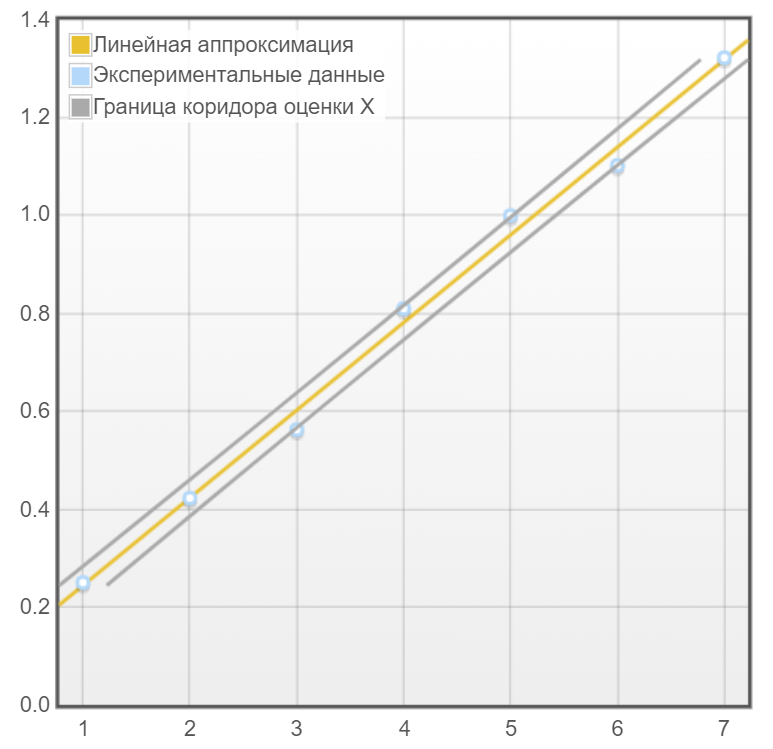
\includegraphics[width = 0.55\textwidth]{гр1.png}
			\caption{Зависимость $r^2(N)$, с погрешностями}
		\end{center}
	\end{figure}

\begin{figure}[h]
		\begin{center}
			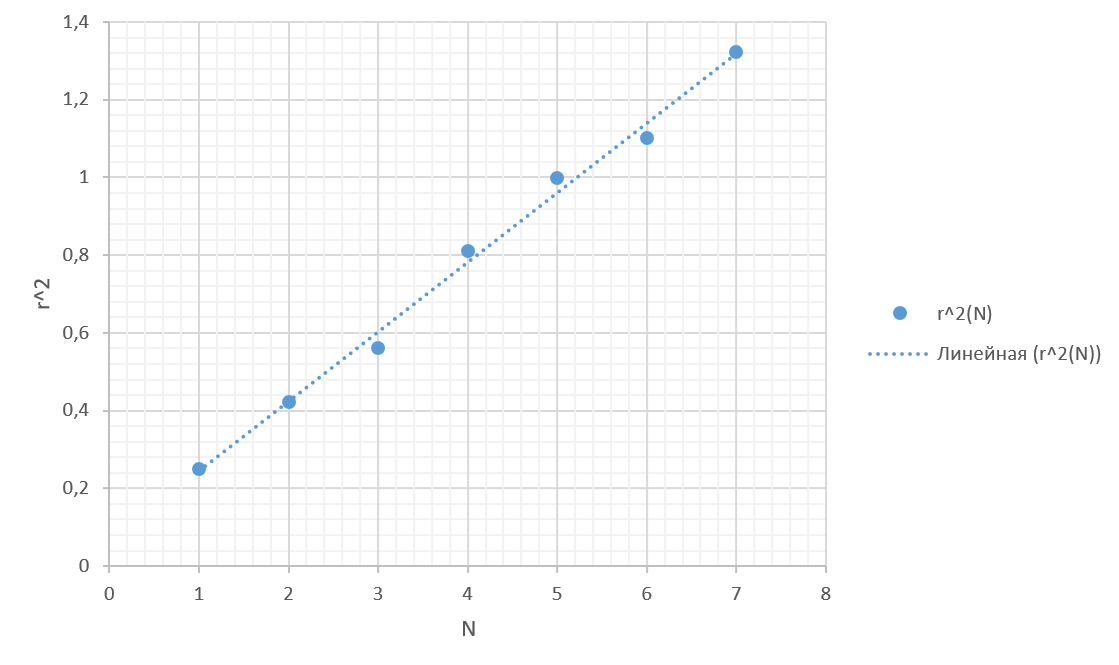
\includegraphics[width = 0.85\textwidth]{гр2.png}
			\caption{Зависимость $r^2(N)$}
		\end{center}
	\end{figure}
	
\newpage

Проверим справедливость формулы

$$
r_n \approx \sqrt{\frac{2 n L(L-a)}{m_0}},
$$

Найдем угловые коэффициенты прямых для каждой установки по МНК.

\[
	a = \frac{<x_i y_i> - < x > < y_i >}{< x_i^2> - < x_i >^2}
\]

\[
	b = < \nu_i > - a < N_i >
\]

Также рассчитаем их погрешности

\begin{equation}
	S_a^2 = \frac{< x_i^2>}{< x_i^2 > - < x_i >^2} \cdot \frac{<  b_i - b > ^2}{n - 2}
\end{equation}

3) Получим зависимость

\begin{equation}
	r_n^2 = (0.065 \pm 0.028) + (0.1791 \pm 0.0062)\cdot n
\end{equation}

Итого $\sqrt{\frac{2 L(L-a)}{m_0}} = 0.179 \pm 0.006$

Тогда $\frac{2 L(L-a)}{m_0} = 0.032 \pm 0.002 \text{ см}^2$

Теоретически, $\frac{2 L(L-a)}{m_0} = 2 \frac{(2 BC + SB + OB)(2 BD + SB + OB)}{2(BC-BD)/\lambda} = 0.028 \text{ см}^2$

В пределах погрешности, величины близки

Расходение может быть обусловлено неточностью выставления a.

4) После смещения зеркала сместим пятно на 1.85 см. Ширина полосы в центре экрана станет $l = \frac{3}{6} = 0.5 \pm 0.1$ мм.

Угол поворота зеркала $\alpha = \frac{OO'}{2 OS_1} \approx 1.2 \pm 0.1 ^\circ$.

Смещение изображения источника света $S_2 S_2' = O O' \frac{S_1 S_2}{OS_1} = \frac{2 (BD-BC)}{2 BC + SB + OB} = 1.7 \pm 0.1$ мм.

5) Отъюстируем систему и уберем линзу II.

\subsection{III. Измерение длины волны лазерного излучения}

1-4) Запустим частотомер в режиме счета импульсов. Запустим 10 прогонов на большой скорости и запишем число колец, прошедших через центр экрана.

\begin{center}
\begin{tabular}{|c|c|c|c|c|c|}
\hline 
N $\cdot 10^3$ & 101707 &
101774 &
101818 &
101738 &
101749 \\
&101644 &
101655 & 
101464 &
101554 &
101554 \\


\hline
\end{tabular}
\end{center}

Усреднив $N = 101670 \pm 40$, получим длину волны лазерного излучения(l = 32 мм)

$$
	\lambda = \frac{2 l}{N} = 629.5 \pm 0.3 \text{ нм} 
$$

Теоретическое значение отличается несильно; $\lambda_\text{теор} = 632.8$ нм.

\subsection{IV. Исследование эффекта Доплера}

1-4) Проведем измерения для 3х различных скоростей двигателя. Результаты после усреднения запишем в таблицу. Для усреднения значения частоты берется медиана выборки, поскольку отклонения от среднего значения часто носят псевдослучайный характер.

\begin{center}
\begin{tabular}{|c|c|c|c|}
\hline
& $\tau$, сек & $\nu_\text{допл}$, Гц & $v_\text{движ}$, мм/с \\
\hline 
1 скорость & $31.25 \pm 0.11$ & $3120 \pm 20$ & $1.024 \pm 0.004$\\
2 скорость & $76.96 \pm 0.05$ & $1291 \pm 6$ & $0.4158 \pm 0.0003$ \\
3 скорость & $218.94 \pm 0.14$ & $720 \pm 20$ & $0.14616 \pm 0.00009$ \\
\hline
\end{tabular}
\end{center}

5) Измерим частоту дрожания картины и найдем медиану выборки.

$\nu_\text{дрож} = 320 \pm 50$ Гц.

Фактически, на 3 скорости скорость двигателя флуктуировала в чуть меньших пределах, но это явно было связано с частотой его вращения, а не с частотой дрожания. Поэтому последней можно пренебречь.

6) Построим график доплеровской частоты в зависимости от скорости
передвижения зеркала

\newpage

\begin{equation}
	v_\text{движ} = \frac{\lambda}{2} \nu_\text{допл}
\end{equation}

\begin{figure}[h]
		\begin{center}
			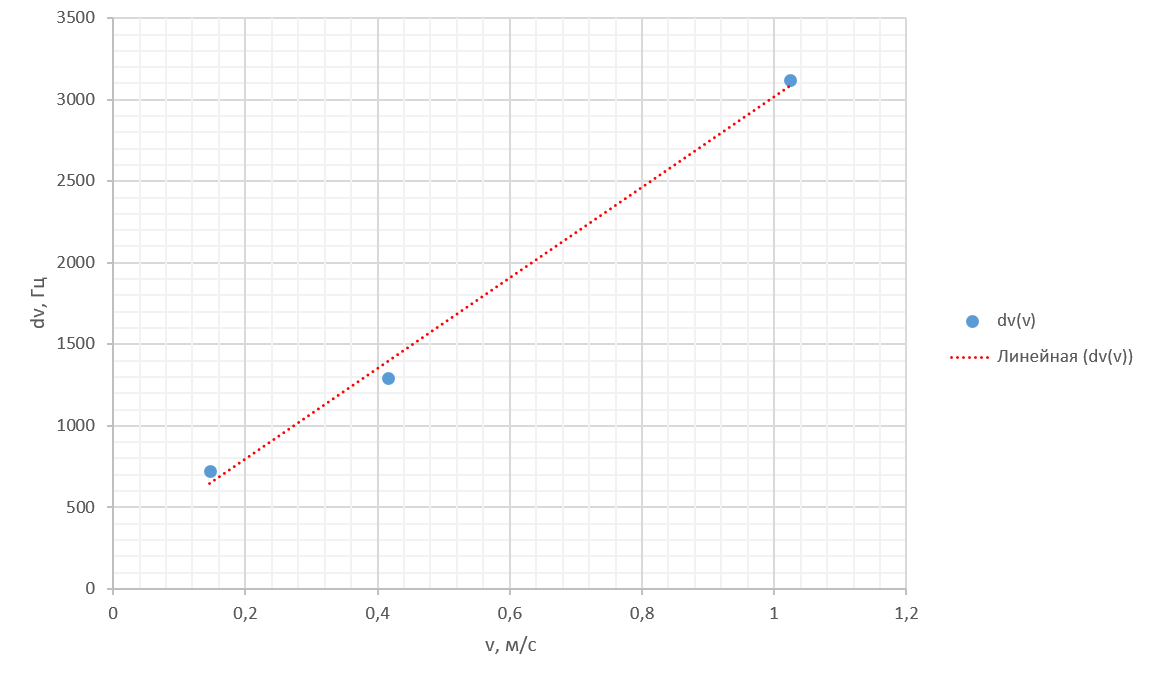
\includegraphics[width = 0.85\textwidth]{гр3.png}
			\caption{Зависимость $\Delta \nu(v)$}
		\end{center}
	\end{figure}
	
Аппроксимация по МНК

\begin{equation}
	v_\text{движ} = (-0.083 \pm 0.053) + (0.000358 \pm 0.000027)\cdot \nu_\text{допл}
\end{equation}

Итого $\lambda_\text{допл} = 720 \pm 50$ нм, что попадает в теоретический диапазон.

7) Выключим установку

%\begin{center}
%\begin{tabular}{|c|c|c|c|}
%\hline 
%\multicolumn{2}{|c|}{$h_\text{ман}$, мм} & $\sigma, \frac{\text{мН}}{\text{К}}$ & T, $^\circ$C \\
%\hline
%188.0 & 188.0 & $(64.5 \pm 3.9)$ & 22\\
%187.0 & 187.0 & $(64.0 \pm 3.9)$ & 30\\
%185.5 & 186.0 & $(63.3 \pm 3.9)$ & 35\\
%184.0 & 184.5 & $(62.5 \pm 3.9)$ & 40\\
%182.5 & 183.0 & $(61.7 \pm 3.9)$ & 45\\
%181.0 & 181.0 & $(60.8 \pm 3.8)$ & 50\\
%179.0 & 179.5 & $(59.9 \pm 3.8)$ & 55\\
%177.5 & 177.5 & $(59.0 \pm 3.8)$ & 60\\
%\hline
%\end{tabular}
%\end{center}

%
%Найдем угловые коэффициенты прямых для каждой установки по МНК.
%
%\[
%	a = \frac{<x_i y_i> - < x > < y_i >}{< x_i^2> - < x_i >^2}
%\]
%
%\[
%	b = < \nu_i > - a < N_i >
%\]
%
%Также рассчитаем их погрешности
%
%\begin{equation}
%	S_a^2 = \frac{< x_i^2>}{< x_i^2 > - < x_i >^2} \cdot \frac{<  b_i - b > ^2}{n - 2}
%\end{equation}


%\begin{center}
%	\Large $q(T)$
%\end{center}

\section{Вывод}

Измерения длины волны методом подсчета колец оказалось значительно точнее метода Доплера. Связано это вероятно с неточностью полученной приборной частоты. Из-за неравномерности вращения двигателя первый метод значительно точнее усредняет флуктуации и дает верный результат.

Цели работы выполнены.

\section{Ресурсы}

Расчет по МНК: метод-наименьших-квадратов.рф


\end{problem}
\end{document}